\section{Evaluation}\label{sec:eval}

For evaluation purposes we implemented two more applications in addition to the
main motivation example - Smart-home and Adaptive protocol. For each application
we compare nesC implementation against its \conesc counterpart.

\begin{table}[!h]
\renewcommand{\arraystretch}{1.3}
\caption{Complexity comparison.}
\label{tab:compres}
\resizebox{\columnwidth}{!}{
  \centering
\begin{tabular}{|l|c|c|c|c|c|c|}
\hline
&&&& \multicolumn{3}{@{\hspace{0.3em}}c@{\hspace{0.3em}}|}
{\bfseries Average per-module}\\[0.1in]
\bfseries Application & \rotatebox{90}{\bfseries LOC} 
& \rotatebox{90}{\pbox{0in}{\bfseries Variable\\declarations}} 
& \rotatebox{90}{\bfseries Functions} & \rotatebox{90}{\bfseries LOC}
& \rotatebox{90}{\pbox{0in}{\bfseries Variable\\declarations}}
& \rotatebox{90}{\bfseries Functions}\\
\hline
\hline
Wildlife tracking -- nesC&456&17&19&48&6&8\\
\hline
Wildlife tracking -- ConesC&539(440)&17&30&26,5&3&2\\
\hline
Wildlife tracking -- generated&1628&--&--&--&--&--\\
\hline
\hline
Smart-home -- nesC&360&24&28&28&2&2\\
\hline
Smart-home -- ConesC&382(289)&24&56&13&0,8&1,9\\
\hline
Smart-home -- generated&1310&--&--&--&--&--\\
\hline
\hline
Adaptive protocol -- nesC&150&10&13&38&2,5&3,25\\
\hline
Adaptive protocol -- ConesC&191(147)&5&21&14,7&0,4&1,6\\
\hline
Adaptive protocol -- generated&636&--&--&--&--&--\\
\hline
\end{tabular}
}
\end{table}

We estimate the complexity of the program by using such metrics as the number of
lines of code (LOC), the number of variables declared and functions
defined~\cite{Pressman01}. Despite our results, which are displayed on
Table~\ref{tab:compres}, show moderate increase of complexity of the whole
application, there is significant reduction in per-module complexity. We believe
that in larger applications the number of the similar lines of code will be
bigger. Moreover, the complexity could be reduced (as shown in
Table~\ref{tab:compres} in parenthesis) by having a tool to generate a
boilerplate code from the diagram, similar to the one displayed in
Fig.~\ref{fig:design}.

Considering the generated code, we conclude that the program written in nesC in
context-oriented style would be more than 3 time bigger than \conesc-written
analog. Our approach makes context-oriented programming as simple as programming
in plain nesC.

\begin{figure}
\centering
\subfloat[CPU overhead.]{
  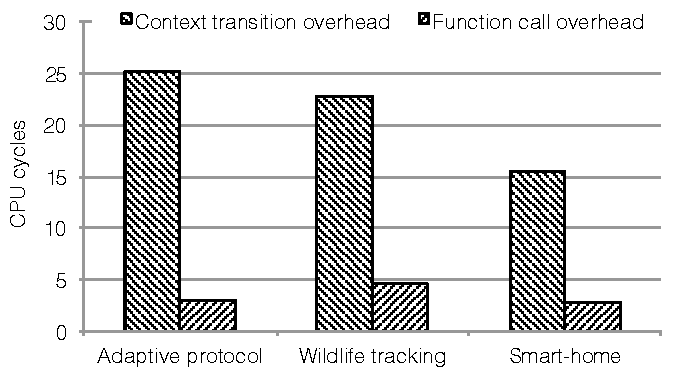
\includegraphics[width =0.5\columnwidth]{imgs/cpu_overhead}
  \label{fig:cpuo}
}
\subfloat[Memory overhead.]{
  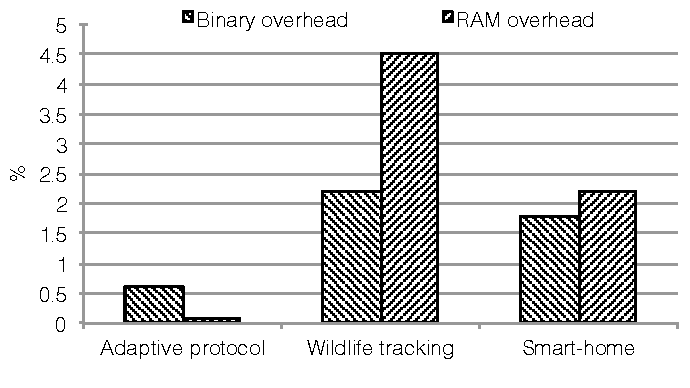
\includegraphics[width=0.5\columnwidth]{imgs/memory_overhead}
  \label{fig:memo}
}
\caption{CPU and memory overhead.}
\label{fig:cmo}
\end{figure}

Figure~\ref{fig:cmo} depicts CPU and memory overhead. The latter is lesser than
2,5\% for binary size and less than 4,5\% for RAM overhead. The average CPU
overhead for layered function calls oscillates from 2 to 5 CPU cycles depending
on application, which is negligible in terms of energy consumption, since the
simplest operation in TinyOS -- turn on/off LEDs -- consumes 8 CPU cycles. The
context transitions overhead is bigger -- from 10 to 25 CPU cycles -- but
remains in the same order of magnitude.
